\chapter{Many Electron Atoms}
%\section{Spin-statisticts theorem}
%Particle with integer spin (bosons) are described by symmetric wave functions, particle with half-integer spins (fermions) are described by anti-symmetric wavefunctions.
%
%Look at $n$ non-interacting identical particles
%\begin{dmath}[]
%	\psi\left( 1,\ldots,N \right)\prod_{i=1}^{N}\psi_i(i)
%\end{dmath}
%\begin{description}
%	\item[bosonic case:]
%		\begin{dmath}[]
%			\psi_S\left( 1,\ldots,N \right)=\sum_{p\in S_N}^{}\psi_1\left( P(1) \right)\ldots \psi_N\left( P(N) \right)
%		\end{dmath}
%	\item[fermionic case] 
%		\begin{dmath}[]
%			\psi_A\left( 1,\ldots,N \right)=\frac{1}{\sqrt{N!}}\sum_{P\in S_N}^{}\left( -1 \right)^{P}\psi_1\left( P(1) \right)\ldots \psi_{N}\left( P(N) \right)
%		\end{dmath}
%		$\psi_A$ can be written as Slater determinant
%\end{description}
%Consider Atom with $N$ electrons
\begin{dmath}[]
	H=\sum_{i=1}^{N}\left( \frac{p^2}{2m}-\frac{Ze^2}{r} \right)+\underbrace{\sum_{i>j}^{}\frac{e^2}{\abs{\vtr{r}_i-\vtr{r}_j}}}_{\footnotemark}
\end{dmath}
\footnotetext{interaction between electrons} $\to$ complicated! we want:
\begin{dmath}[]
	H\psi\left( 1,\ldots,N \right)=E\psi\left( 1,\ldots,N \right)
\end{dmath}
\section{Identical particles}
Consider $N$ identical particles $H\left( 1,..,N \right)$ wave function $\psi\left( 1,\cdots,N \right)$.

In classical mechanics we can always distinguish these $n$ particles state.
\begin{figure}[]
	\begin{center}
		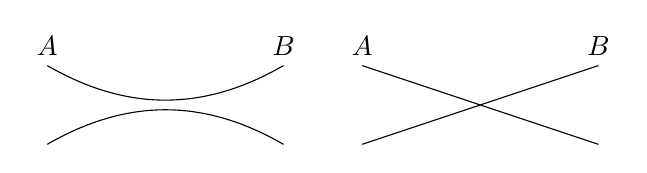
\begin{tikzpicture}[scale=0.5]
			\coordinate[label=above:$A$] (a) at (-3,1);
			\coordinate[label=above:$B$] (b) at (3,1);
			\coordinate[] (a2) at (-3,-1);
			\coordinate[] (b2) at (3,-1);
			\path[draw] (a) to[bend right] node{} (b);
			\path[draw] (a2) to[bend left] node{} (b2);
			\begin{scope}[xshift=8cm]
				\coordinate[label=above:$A$] (a) at (-3,1);
				\coordinate[label=above:$B$] (b) at (3,1);
				\coordinate[] (a2) at (-3,-1);
				\coordinate[] (b2) at (3,-1);
				\draw[] (a) -- (b2);
				\draw[] (a2) -- (b);
			\end{scope}
		\end{tikzpicture}
	\end{center}
	\caption{}
	\label{fig:}
\end{figure}
In Quantum Mechanics, we cannot keep track of individual particles if their wave functions overlap. Defin permutation operator $P_{ij}$ interchanging $i$ and $j$
\begin{dgroup}[]
	\begin{dmath}[]
		P_{ij}\psi\left( 1,\ldots,i,\ldots,j,\ldots,N \right)=\psi\left( 1,\ldots,j,\ldots,i,\ldots,N \right)
	\end{dmath}
	\begin{dmath}[]
		P_{ij}^2=1
	\end{dmath}
	\begin{dmath}[]
		\hiderel{\Rightarrow} \text{evals }\pm 1
	\end{dmath}
\end{dgroup}
$H$ must be invariant under $i\leftrightarrow j$
\begin{dmath}[]
	\hiderel{\Rightarrow}\comm{H}{P_{ij}}=0
\end{dmath}
There are $N!$ permutations of elements $1\cdots N$, they fall into two classes, even and odd:
\begin{dmath}[]
	\sgn(P)=
	\begin{cases}
		+1&\left( -1 \right)^2 \text{even nr. of Interchanges}\\
		-1&\left( -1 \right)^2 \text{odd nr. of Interchanges}
	\end{cases}
\end{dmath}
we have $\comm{H}{P}$.
$P$ is unitary since
\begin{dgroup}[]
	\begin{dmath}[]
		\braket{\chi}{\psi}=\braket{P\xi}{P\psi}=\mel{\xi}{P^{\dagger}P}{\psi}
	\end{dmath}
	\begin{dmath}[]
		\hiderel{\Rightarrow} P^{\dagger}P=1
	\end{dmath}
	\begin{dsuspend}
		for any observable $A$ we have
	\end{dsuspend}
	\begin{dmath}[]
		\comm{A}{P}=0
	\end{dmath}.
\end{dgroup}
(\emph{Identical} part) two combinations are important:
\begin{enumerate}[i)]
	\item totally symmetric $\ket{\psi}_S$ with
		\begin{dmath}[]
			P\ket{\psi}_S=\ket{\psi}_S
		\end{dmath}
		with $\ket{\psi}_S$ completely symmetric linear combination of all $N!$ Permutations.
	\item totally antisymmetric $\ket{\psi}_A$ with 
		\begin{dmath}[]
			P\ket{\psi}_A=\left( -1 \right)^P\ket{\psi}_A
		\end{dmath}
\end{enumerate}
\paragraph{Example} $N=3$
\begin{dgroup}[]
	\begin{dmath}[]
		\ket{\psi}_S=\frac{1}{\sqrt{3!}}\left( \psi\left( 1,2,3 \right)+\psi\left( 2,1,3 \right)+\psi\left( 1,3,2 \right)+\psi\left( 2,3,1 \right)+\psi\left( 3,1,2 \right)+\psi\left( 3,2,1 \right) \right)
	\end{dmath}
	\begin{dmath}[]
		\ket{\psi}_A=\frac{1}{\sqrt{3!}}\left( \psi\left( 1,2,3 \right)+\psi\left( 2,3,1 \right)+\psi\left( 3,2,1 \right)-\psi\left( 2,1,3 \right)-\psi\left( 3,2,1 \right)-\psi\left( 1,3,2 \right) \right)
	\end{dmath}
\end{dgroup}
\paragraph{spin-statistics theorem}
particles with \emph{integer spin} (bosons) are described by \emph{symmetric} wave-functions\\
particles with \emph{half-integer spin} (fermions) are described by \emph{antisymmetric} wave functions
\begin{dgroup}[]
	\begin{dsuspend}
		Bosonic case:
	\end{dsuspend}
	\begin{dmath}[]
		\psi_S\left( 1,\ldots,N \right)=\frac{1}{\sqrt{N!}}\sum_{p\in S_n}^{}\psi_1\left( P(1) \right)\ldots \psi_N\left( P(N) \right)
	\end{dmath}
	\begin{dsuspend}
		fermionic case
	\end{dsuspend}
	\begin{dmath}[]
		\psi_A\left( 1,\ldots,N \right)=\frac{1}{\sqrt{N!}}\sum_{p\in S_n}^{}\left( -1 \right)^P\psi_1\left( P(1) \right)\ldots \psi_N\left( P(N) \right)
	\end{dmath}
	\begin{dsuspend}
		$\psi_A$ can be written as a Slater determinant
	\end{dsuspend}
	\begin{dmath}[]
		\psi_A\left( 1,\ldots,N \right)=\frac{1}{\sqrt{N!}}\det
		\begin{pmatrix}
			\psi_1(1)&\cdots&\psi_1(N)\\
			\vdots&\ddots&\vdots\\
			\psi_N(1)&\cdots&\psi_N(N)
		\end{pmatrix}
	\end{dmath}
\end{dgroup}
\paragraph{Pauli exclusion principle}
Two identical fermions (same quantum number, $\vtr{s}$,\ldots) cannot be at the same position. Wave function vanishes for $r_i,r_j;s_i=s_j,\cdots$. i.e. $1=2$ $\to$ Fermi gas.
\section{Thomas-Fermi approximation}
$\simeq$ semi classical: assume each electron feels average potential $\Phi(r)$, (spherically symmetric)
\begin{dmath}[]
	V=-\frac{Ze^2}{r}\xrightarrow{\text{other electron}}-e\Phi(r)
\end{dmath}
Poisson equation:
\begin{dmath}[]
	\vtr{\nabla}^2\Phi=-4\pi\tilde{\rho}\stackrel{r>0}{=}4\pi e\rho(r)
\end{dmath}
total charge density (other electron and nucleus)
\begin{dmath}[]
	\tilde{\rho}=-e\rho(r)+Ze\delta(r)
\end{dmath}
find relation between $\rho$ and $\Phi$. Let $n$ be nr. states in certain energy range
\begin{dgroup}[]
	\begin{dmath}[]
		n=\frac{2}{\left( 2\pi\hbar \right)^3}\condition*{\ds\text{if }E=\frac{p^2}{2m}-e\Phi<0}
	\end{dmath}
	\begin{dmath}[]
		n=0\condition*{\text{if }E=\frac{p^2}{2m}-e\Phi>0}
	\end{dmath}
	\begin{dmath}[]
		\rho=\int_{0}^{\sqrt{2me\Phi}}\rd^3 p n=\frac{\left( 4\pi \right)2}{\left( 2\pi\hbar \right)^3}\int_{0}^{\sqrt{2me\phi}}
	\end{dmath}
\end{dgroup}
plug this into Poisson $\to$ differential equation for $\Phi$
\begin{dmath}[]
	\vtr{\nabla}^2\Phi=\frac{1}{R}\dvt{}{r}r\Phi(r)=\frac{32\pi^2 e}{3\left( 2\pi\hbar \right)^3}\left( 2me\Phi \right)^{3/2}
\end{dmath}
solve numerically. boundary condition:
\begin{dgroup}[]
	\begin{dmath}[]
		\phi(r)\to\frac{Ze}{r}\condition{for $r\to 0$}
	\end{dmath}
	\begin{dsuspend}
		normalize
	\end{dsuspend}
	\begin{dmath}[]
		4\pi\int_{}^{}\dd{r}\,\rho(r)r^2=Z
	\end{dmath}
\end{dgroup}
$\leadsto$ ``radius'' of atom (contains all but one electron)
\begin{dmath}[]
	\overline{R}\simeq \text{consant} a Z^{1/3}
\end{dmath}
\section{The Hartree approximation}
Assume 
\begin{dgroup}[]
	\begin{dmath}[]
		\psi\left( 1\ldots N \right)=\varphi_{1}(1)\ldots \varphi_{N}(N)
	\end{dmath}
	\begin{dsuspend}
		as solution to
	\end{dsuspend}
	\begin{dmath}[]
		H\psi=E\psi
	\end{dmath}
	\begin{dsuspend}
		with
	\end{dsuspend}
	\begin{dmath}[]
		H=\sum_{i}^{}\left( \frac{p_{i}^{2}}{2m}-\frac{Ze^2}{r_i} \right)+\sum_{i>j}^{}\frac{e^2}{\abs{\vtr{r}_i-\vtr{r}_j}}
	\end{dmath}
\end{dgroup}
let $\varphi_i$ be distinct and orthogonal (partially taking into account Pauli principle) and normalized
\begin{dmath}[]
	\int_{}^{}\rd^3 r_i\abs{\varphi_i(r_i)}^2=1
\end{dmath}
Want to find stationary state with respect to variation in $\varphi_i$ taking into account normalization via Lagrange multipliers $\varepsilon_i$
\begin{dmath}[]
	\left\langle H \right\rangle=\sum_{i}^{}\int_{}^{}\rd^3\vtr{r}\, \left( \varphi_{i}^{*}(\vtr{r})\left( -\frac{\hbar^2}{2m}\vtr{\nabla}^2-\frac{Ze^2}{r} \right)\varphi_i(r) \right)
	+\sum_{i>j}^{}\int_{}^{}\rd^3 \vtr{r}\int_{}^{}\rd^3 \vtr{r}\, \varphi_{i}^{*}(\vtr{r})\varphi_{j}^{*}(\vtr{r})\frac{e^2}{\abs{\vtr{r}-\vtr{r}'}}\varphi_i(r)\varphi_j(r')
	+\sum_{i}^{}\varepsilon_i\left( \int_{}^{}\rd^3 r\, \abs{\varphi_i(r)}^2 -1\right)
\end{dmath}
take functional derivative $\fdv{}{\varphi_i^*}$
\begin{dgroup}[]
	\begin{dmath}[label=eq:hartree1]
		\left( -\frac{\hbar}{2m}\nabla^2-\frac{Ze^2}{r} \right)\varphi_i
		+V_i(r)\varphi_i(r)=\varepsilon_i\varphi_i(r)
	\end{dmath}
	\begin{dmath}[label=eq:hartree2]
		V_i(r)=\sum_{j\not=i}^{}\int_{}^{}\rd^3 r'\, \frac{e^2}{\abs{\vtr{r}-\vtr{r}'}}\abs{\varphi_j(\vtr{r}')}^2
	\end{dmath}
\end{dgroup}
interaction of $i$-th electron with potential caused by all other ($j\neq i$) electrons

$\varepsilon_i$: ionization energy of $i$-ith electron.
